% !TEX program = pdflatex
% Soutenance — Classification d'images rétiniennes (IFT 3395/6390)
% Compilation (2 passes) :
%   cd slides && pdflatex presentation.tex && pdflatex presentation.tex
\documentclass[10pt,aspectratio=169,professionalfonts]{beamer}

\usepackage[utf8]{inputenc}
\usepackage[T1]{fontenc}
\usepackage[french]{babel}
\usepackage{lmodern}
\usepackage{microtype}
\usepackage{amsmath, amssymb}
\usepackage{graphicx}
\usepackage{booktabs}
\usepackage{array}
\usepackage{xcolor}
\usepackage{tikz}
\usetikzlibrary{positioning, arrows.meta, calc, shadows.blur, shapes.geometric, fit, backgrounds}
\usepackage{hyperref}

% =====================================================================
% THÈME, COULEURS, TYPO
% =====================================================================
\usetheme{Boadilla}
\usefonttheme{structurebold}
\setbeamertemplate{navigation symbols}{}
\setbeamertemplate{itemize items}[circle]
\setbeamertemplate{enumerate items}[default]
\setbeamercovered{transparent}

% --- Palette projet ----------------------------------------------------
\definecolor{Brand}{HTML}{4F46E5}
\definecolor{BrandDark}{HTML}{312E81}
\definecolor{BrandLight}{HTML}{EEF2FF}
\definecolor{Accent}{HTML}{EC4899}
\definecolor{Success}{HTML}{059669}
\definecolor{Warning}{HTML}{D97706}
\definecolor{Danger}{HTML}{DC2626}
\definecolor{Ink}{HTML}{0F172A}
\definecolor{Muted}{HTML}{64748B}

\setbeamercolor{structure}{fg=Brand}
\setbeamercolor{normal text}{fg=Ink}
\setbeamercolor{frametitle}{bg=BrandDark, fg=white}
\setbeamercolor{title}{fg=BrandDark}
\setbeamercolor{subtitle}{fg=Brand!85!black}
\setbeamercolor{block title}{bg=BrandLight, fg=BrandDark}
\setbeamercolor{block body}{bg=BrandLight!40!white, fg=Ink}
\setbeamercolor{block title alerted}{bg=Warning!90!black, fg=white}
\setbeamercolor{block body alerted}{bg=Warning!7, fg=Ink}
\setbeamercolor{block title example}{bg=Success!85!black, fg=white}
\setbeamercolor{block body example}{bg=Success!7, fg=Ink}

\hypersetup{colorlinks=true, linkcolor=BrandDark, urlcolor=Brand, citecolor=BrandDark}

\setbeamerfont{title}{size=\LARGE, series=\bfseries}
\setbeamerfont{subtitle}{size=\normalsize, series=\mdseries}
\setbeamerfont{frametitle}{size=\large, series=\bfseries}
\setbeamerfont{footline}{size=\tiny}

% =====================================================================
% PIED DE PAGE AVEC BARRE DE PROGRESSION
% =====================================================================
\setbeamertemplate{footline}{%
  \leavevmode%
  \begin{tikzpicture}
    \useasboundingbox (0,0) rectangle (\paperwidth,2pt);
    \fill[BrandDark!10] (0,0) rectangle (\paperwidth,1.6pt);
    \ifnum\inserttotalframenumber>0\relax
      \pgfmathparse{\insertframenumber/\inserttotalframenumber}%
      \fill[Brand] (0,0) rectangle (\pgfmathresult\paperwidth,1.6pt);%
    \fi
  \end{tikzpicture}\par
  \vspace{0.2em}
  \hbox{%
    \begin{beamercolorbox}[wd=.35\paperwidth,ht=2.2ex,dp=1ex,leftskip=1em]{author in head/foot}%
      \tiny\color{Muted}\insertshortauthor%
    \end{beamercolorbox}%
    \begin{beamercolorbox}[wd=.45\paperwidth,ht=2.2ex,dp=1ex,center]{title in head/foot}%
      \tiny\color{Muted}\insertshorttitle%
    \end{beamercolorbox}%
    \begin{beamercolorbox}[wd=.2\paperwidth,ht=2.2ex,dp=1ex,rightskip=1em]{page number in head/foot}%
      \hfill\tiny\color{Muted}\insertframenumber\,/\,\inserttotalframenumber%
    \end{beamercolorbox}%
  }%
}

% =====================================================================
% MACROS RÉUTILISABLES
% =====================================================================
\graphicspath{{../assets/}}

% Carte statistique : \statcard{valeur}{libellé}{couleur}
\newcommand{\statcard}[3]{%
  \begin{tikzpicture}[baseline]
    \node[draw=#3, line width=1pt, rounded corners=4pt,
          fill=#3!8, text=Ink, minimum width=2.5cm, minimum height=1.4cm,
          align=center, inner sep=4pt, blur shadow={shadow blur steps=4, shadow opacity=18, shadow xshift=0pt, shadow yshift=-1pt}]
    {\textbf{\Large\color{#3}#1}\\[-0.1em]\scriptsize\color{Muted}#2};
  \end{tikzpicture}%
}

% Puce colorée : \bpoint{couleur} ...
\newcommand{\bpoint}[1]{\item[\textcolor{#1}{$\blacktriangleright$}]}

% =====================================================================
% MÉTADONNÉES
% =====================================================================
\title[Retinal DL]{Classification d'images rétiniennes\\par apprentissage profond}
\subtitle{Deep Learning · Compétition Kaggle 2}
\author[Jegham · Ben Mansour]{Jegham Mohamed \quad \textbar\quad Ben Mansour Louay}
\institute[]{Polytechnique Sousse}
\date{}

\begin{document}

% =====================================================================
% SLIDE 1 — TITRE
% =====================================================================
\begin{frame}[plain,noframenumbering]
  \begin{tikzpicture}[overlay, remember picture]
    % Bande verticale décorative gauche
    \fill[Brand] (current page.south west) rectangle ([xshift=0.6cm]current page.north west);
    \fill[Accent] ([xshift=0.6cm]current page.south west) rectangle ([xshift=0.7cm]current page.north west);
  \end{tikzpicture}

  \vspace*{0.6em}
  \begin{center}
    {\tiny\color{Muted}\textsc{Soutenance · projet final}}\\[0.4em]
    {\usebeamercolor[fg]{title}\usebeamerfont{title}\inserttitle\par}
    \vspace{0.5em}
    {\usebeamercolor[fg]{subtitle}\usebeamerfont{subtitle}\insertsubtitle\par}
    \vspace{1.4em}
    \rule{0.42\textwidth}{0.6pt}\\[0.9em]
    {\normalsize\insertauthor}\\[0.35em]
    {\small\color{Muted}\insertinstitute}
  \end{center}

  \vfill
  \begin{center}
    \statcard{1\,080}{images d'entraînement}{Brand}\quad
    \statcard{5}{classes de qualité}{Accent}\quad
    \statcard{4}{architectures comparées}{Success}\quad
    \statcard{$+2$}{bonus Streamlit}{Warning}
  \end{center}
  \vspace*{1.4em}
\end{frame}

% =====================================================================
% SLIDE 2 — PROBLÈME ET DONNÉES
% =====================================================================
\begin{frame}{Problème et données}
  \begin{columns}[T,onlytextwidth]
    \column{0.58\textwidth}
    \textbf{Objectif.}\quad Estimer automatiquement la \alert{qualité perceptive} d'une image rétinienne parmi \textbf{5 classes} ordonnées (0 = la plus basse $\rightarrow$ 4 = la plus haute).

    \medskip
    \textbf{Jeu de données.}
    \begin{itemize}\setlength\itemsep{0.25em}
      \item \textbf{Entraînement :} 1\,080 images RVB $28{\times}28$
      \item \textbf{Test public (Kaggle) :} 400 images
      \item Classes \textit{déséquilibrées} $\rightarrow$ split \textbf{stratifié}
      \item \textit{Petit jeu} $\rightarrow$ risque \alert{élevé de surapprentissage}
    \end{itemize}

    \medskip
    \textbf{Métriques.}\quad Accuracy · \textbf{F1 macro} · matrice de confusion · \textbf{ROC} multiclasse (one-vs-rest, AUC macro).

    \column{0.42\textwidth}
    \centering
    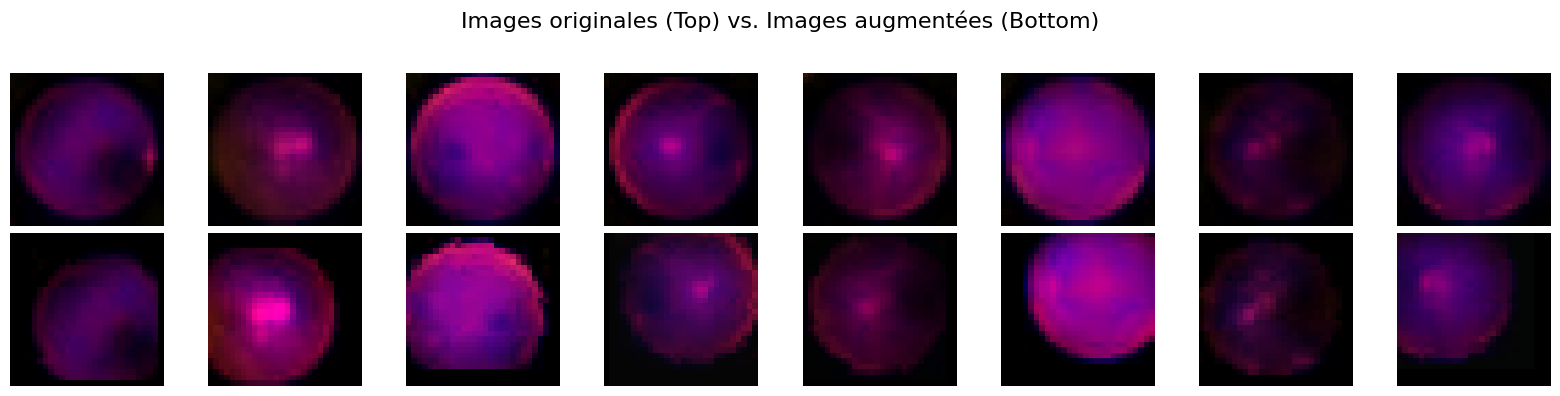
\includegraphics[width=0.96\linewidth]{augmentation_data.png}\\[-0.2em]
    {\scriptsize\color{Muted}\textit{Exemples originaux (haut) vs.\ augmentés (bas)}}
  \end{columns}
\end{frame}

% =====================================================================
% SLIDE 3 — PIPELINE
% =====================================================================
\begin{frame}{Pipeline Deep Learning}
  \vspace{-0.2em}
  \centering
  \resizebox{\linewidth}{!}{%
    \begin{tikzpicture}[
      font=\small\sffamily,
      node distance=0.55cm and 0.50cm,
      box/.style={
        draw=Brand, line width=0.9pt, rounded corners=4pt,
        minimum width=2.5cm, minimum height=1.25cm,
        align=center, fill=Brand!6, text=BrandDark,
        blur shadow={shadow blur steps=4, shadow opacity=15, shadow xshift=0pt, shadow yshift=-1pt}
      },
      arr/.style={-{Stealth[length=3mm,width=2.6mm]}, line width=1.1pt, BrandDark!75}
    ]
      \node[box] (data) {\textbf{Données}\\[-0.1em]\scriptsize Pickle · 1080 imgs};
      \node[box, right=of data] (prep) {\textbf{Prétraitement}\\[-0.1em]\scriptsize $/255$ · tenseurs};
      \node[box, right=of prep] (aug)  {\textbf{Augmentation}\\[-0.1em]\scriptsize $\times 5$ à $\times 15$};
      \node[box, right=of aug]  (mdl)  {\textbf{Modèle DL}\\[-0.1em]\scriptsize MLP / CNN / ResNet};
      \node[box, right=of mdl]  (out)  {\textbf{Sortie}\\[-0.1em]\scriptsize logits · softmax};
      \foreach \a/\b in {data/prep, prep/aug, aug/mdl, mdl/out}{\draw[arr] (\a) -- (\b);}
    \end{tikzpicture}%
  }

  \vspace{0.7em}
  \begin{itemize}\setlength\itemsep{0.30em}
    \bpoint{Brand} \textbf{Augmentation} : flip, rotation, recadrage, ColorJitter, affine, equalize, sharpness.
    \bpoint{Brand} \textbf{Régularisation} : BatchNorm, Dropout, weight decay, \textbf{early stopping} sur la val.\ loss.
    \bpoint{Brand} \textbf{Optimisation} : Adam ou SGD + momentum, \textbf{ReduceLROnPlateau}, \texttt{CrossEntropyLoss} (label smoothing).
    \bpoint{Brand} \textbf{Validation} : découpage stratifié 80/20, meilleurs poids rechargés après entraînement.
  \end{itemize}
\end{frame}

% =====================================================================
% SLIDE 4 — ARCHITECTURE CNN
% =====================================================================
\begin{frame}{Architecture principale : \textsc{cnn} compacte}
  \vspace{-0.2em}

  %--- Diagramme horizontal : flux des feature maps ----------------------
  \centering
  \resizebox{\linewidth}{!}{%
    \begin{tikzpicture}[
      font=\footnotesize\sffamily,
      every node/.style={align=center, inner sep=3pt},
      input/.style={
        draw=Muted, line width=0.7pt, rounded corners=3pt,
        fill=Muted!15, text=Ink,
        minimum width=1.05cm
      },
      conv/.style={
        draw=Brand, line width=0.7pt, rounded corners=3pt,
        fill=Brand!12, text=BrandDark,
        minimum width=1.05cm
      },
      pool/.style={
        draw=Accent, line width=0.7pt, rounded corners=3pt,
        fill=Accent!18, text=Accent!50!black,
        minimum width=0.85cm
      },
      head/.style={
        draw=Success, line width=0.7pt, rounded corners=3pt,
        fill=Success!15, text=Success!40!black,
        minimum width=1.05cm
      },
      out/.style={
        draw=Warning, line width=0.9pt, rounded corners=3pt,
        fill=Warning!22, text=Warning!50!black,
        minimum width=1.05cm
      },
      arr/.style={-{Stealth[length=1.8mm]}, BrandDark!70, line width=0.8pt},
      sz/.style={font=\tiny\color{Muted}, inner sep=2pt}
    ]
      % Bloc 1 : extraction (haute résolution 28x28)
      \node[input, minimum height=1.9cm]                       (in) {\textbf{Image}\\[-0.1em]\scriptsize RVB};
      \node[conv,  minimum height=1.9cm, right=0.22cm of in]   (c1) {\textbf{Conv}\\[-0.1em]$3{\times}3$\,/\,32};
      \node[conv,  minimum height=1.9cm, right=0.10cm of c1]   (c2) {\textbf{Conv}\\[-0.1em]$3{\times}3$\,/\,32};
      \node[pool,  minimum height=1.5cm, right=0.10cm of c2]   (p1) {\textbf{Max}\\[-0.1em]\textbf{Pool}};

      % Bloc 2 : extraction (résolution réduite 14x14)
      \node[conv,  minimum height=1.5cm, right=0.28cm of p1]   (c3) {\textbf{Conv}\\[-0.1em]$3{\times}3$\,/\,64};
      \node[conv,  minimum height=1.5cm, right=0.10cm of c3]   (c4) {\textbf{Conv}\\[-0.1em]$3{\times}3$\,/\,128};
      \node[pool,  minimum height=1.0cm, right=0.10cm of c4]   (p2) {\textbf{Max}\\[-0.1em]\textbf{Pool}};

      % Tête de classification
      \node[head,  minimum height=1.0cm, right=0.36cm of p2]   (fl) {\textbf{Flatten}\\[-0.1em]\scriptsize $6272$};
      \node[head,  minimum height=1.0cm, right=0.12cm of fl]   (fc) {\textbf{FC 128}\\[-0.1em]\scriptsize +BN+Drop.};
      \node[out,   minimum height=0.85cm,right=0.18cm of fc]   (sm) {\textbf{FC 5}\\[-0.1em]\scriptsize softmax};

      % Flèches de flux
      \foreach \a/\b in {in/c1,c1/c2,c2/p1,p1/c3,c3/c4,c4/p2,p2/fl,fl/fc,fc/sm}{%
        \draw[arr] (\a.east) -- (\b.west);}

      % Dimensions des feature maps sous chaque colonne
      \node[sz, below=2pt of in.south] {$28{\times}28{\times}3$};
      \node[sz, below=2pt of c2.south] {$28{\times}28{\times}32$};
      \node[sz, below=2pt of p1.south] {$14{\times}14{\times}32$};
      \node[sz, below=2pt of c4.south] {$14{\times}14{\times}128$};
      \node[sz, below=2pt of p2.south] {$7{\times}7{\times}128$};
      \node[sz, below=2pt of fl.south] {$6272$};
      \node[sz, below=2pt of fc.south] {$128$};
      \node[sz, below=2pt of sm.south] {$5$};

      % Bandeaux de regroupement (Bloc 1 / Bloc 2 / Tête)
      \begin{scope}[on background layer]
        \node[draw=Brand!55, dashed, line width=0.5pt, rounded corners=3pt,
              fill=Brand!5, inner sep=5pt,
              fit=(c1)(p1),
              label={[font=\scriptsize\color{Brand}\bfseries, yshift=-0.4em]above:Bloc 1 — extraction}] {};
        \node[draw=Brand!55, dashed, line width=0.5pt, rounded corners=3pt,
              fill=Brand!5, inner sep=5pt,
              fit=(c3)(p2),
              label={[font=\scriptsize\color{Brand}\bfseries, yshift=-0.4em]above:Bloc 2 — extraction}] {};
        \node[draw=Success!55, dashed, line width=0.5pt, rounded corners=3pt,
              fill=Success!6, inner sep=5pt,
              fit=(fl)(sm),
              label={[font=\scriptsize\color{Success!45!black}\bfseries, yshift=-0.4em]above:Tête — classifier}] {};
      \end{scope}
    \end{tikzpicture}%
  }

  \vspace{0.6em}

  %--- Bande d'hyperparamètres (chips) -----------------------------------
  \begin{center}
    \begin{tikzpicture}[
      font=\scriptsize\sffamily,
      chip/.style={
        draw=Brand!55!black, line width=0.5pt, rounded corners=10pt,
        fill=Brand!12, text=Brand!35!black,
        minimum height=0.55cm, inner xsep=8pt, inner ysep=2pt
      },
      chipOk/.style={
        chip, draw=Success!55!black, fill=Success!15, text=Success!35!black
      }
    ]
      \node[chip]                              (a) {\textbf{Perte}\;\; entropie croisée};
      \node[chip,    right=0.22cm of a]        (b) {\textbf{Optim.}\;\; Adam / SGD};
      \node[chip,    right=0.22cm of b]        (c) {\textbf{lr}\;\; $10^{-3}$};
      \node[chip,    right=0.22cm of c]        (d) {\textbf{wd}\;\; $10^{-4}$};
      \node[chipOk,  right=0.22cm of d]        (e) {$\sim 0{,}9\,\mathrm{M}$ paramètres};
    \end{tikzpicture}
  \end{center}

  \vspace{0.25em}
  \begin{center}
    {\scriptsize\color{Muted}\textit{La hauteur des blocs reflète la résolution spatiale ;\;
      les groupes en pointillés mettent en évidence les trois étages de la \textsc{cnn}.\;
      Inspirée de}~%
      \href{https://www.nature.com/articles/s41598-025-87171-9}{\color{Brand}\texttt{Nature 41598-025-87171-9}}.}
  \end{center}
\end{frame}

% =====================================================================
% SLIDE 5 — COMPARAISON DES MODÈLES
% =====================================================================
\begin{frame}{Comparaison des architectures}
  \vspace{-0.4em}
  \begin{center}
    \footnotesize
    \renewcommand{\arraystretch}{1.30}
    \setlength{\tabcolsep}{6pt}
    \begin{tabular}{@{}l r c c c@{}}
      \toprule
      \textbf{Modèle} & \textbf{\# param.} & \textbf{Train acc.} & \textbf{Val acc.} & \textbf{Test Kaggle} \\
      \midrule
      \textsc{mlp} baseline                & $\sim 1{,}4\,\mathrm{M}$ & 0{,}62 & 0{,}45 & --- \\
      Kernel SVM (référence)               & ---                      & ---    & ---    & 0{,}46 \\
      \textbf{\textcolor{Brand}{\textsc{cnn} (production)}} & $\mathbf{\sim 0{,}9\,M}$ & \textbf{0{,}53} & \textbf{0{,}51} & \textbf{0{,}52} \\
      Small \textsc{resnet}                & $\sim 1{,}1\,\mathrm{M}$ & 0{,}58 & 0{,}50 & --- \\
      \textsc{resnet18} TL (ImageNet)      & $\sim 11\,\mathrm{M}$    & \textit{à compléter} & \textit{à compléter} & \textit{à compléter} \\
      \bottomrule
    \end{tabular}
  \end{center}

  \vspace{0.5em}
  \begin{itemize}\small\setlength\itemsep{0.30em}
    \bpoint{Success} \textbf{\textsc{cnn}} : meilleur compromis \emph{précision · coût · surapprentissage} sur ce dataset.
    \bpoint{Warning} \textbf{\textsc{mlp}} : pas de prior spatial $\rightarrow$ gap train--val très marqué.
    \bpoint{Warning} \textbf{ResNet scratch} : skip connections utiles mais gains limités quand $|\mathcal{D}|$ est faible.
    \bpoint{Brand}   \textbf{\textsc{resnet18} TL} : transfer learning sur ImageNet ; chiffres à reporter depuis \texttt{output/comparison\_table.md}.
  \end{itemize}
\end{frame}

% =====================================================================
% SLIDE 6 — COURBES D'APPRENTISSAGE
% =====================================================================
\begin{frame}{Courbes d'apprentissage \& surapprentissage}
  \begin{columns}[T,onlytextwidth]
    \column{0.55\textwidth}
    \centering
    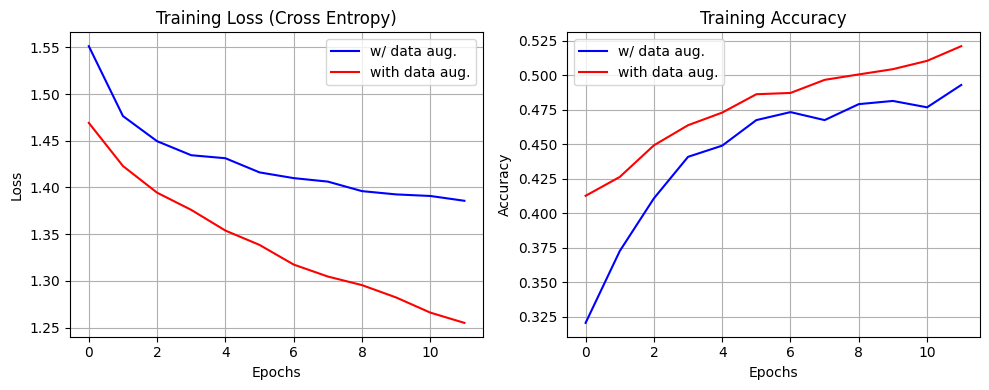
\includegraphics[width=\linewidth]{train_loss_and_error.png}\\[-0.15em]
    {\scriptsize\color{Muted}\textit{Perte et accuracy — sans augmentation (bleu) vs.\ avec (rouge)}}

    \column{0.45\textwidth}
    \begin{itemize}\small\setlength\itemsep{0.35em}
      \bpoint{Danger}  \textbf{Sans augmentation} : train chute, val.\ stagne $\rightarrow$ \alert{surapprentissage} clair.
      \bpoint{Success} \textbf{Avec augmentation} ($\times 10$) : val.\ proche de train $\rightarrow$ meilleure généralisation.
      \bpoint{Brand}   \textbf{Early stopping} déclenché vers les epochs 10--12 selon les runs.
      \bpoint{Brand}   \textbf{BN + Dropout} stabilisent l'optimisation et réduisent la variance.
    \end{itemize}
  \end{columns}
\end{frame}

% =====================================================================
% SLIDE 7 — MATRICES DE CONFUSION
% =====================================================================
\begin{frame}{Matrices de confusion}
  \begin{columns}[T,onlytextwidth]
    \column{0.5\textwidth}
    \centering
    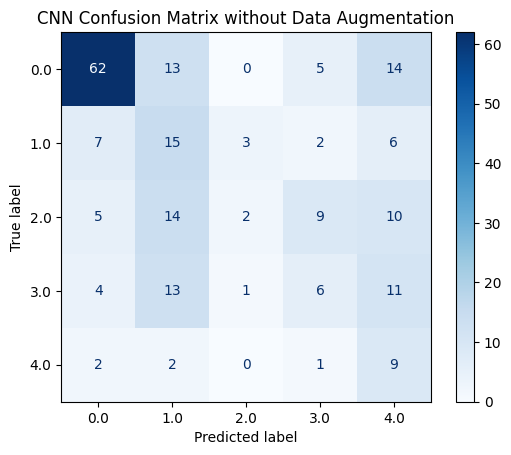
\includegraphics[width=0.94\linewidth]{conf_matrix_without_data_aug.png}\\[-0.1em]
    {\scriptsize\color{Muted}\textit{Sans augmentation}}

    \column{0.5\textwidth}
    \centering
    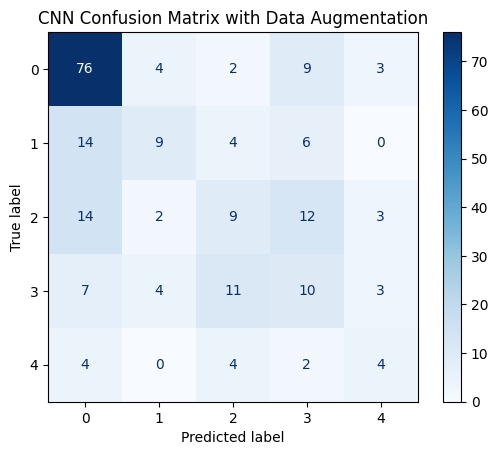
\includegraphics[width=0.94\linewidth]{conf_matrix_with_data_aug.png}\\[-0.1em]
    {\scriptsize\color{Muted}\textit{Avec augmentation}}
  \end{columns}

  \vspace{0.4em}
  \begin{itemize}\small\setlength\itemsep{0.25em}
    \bpoint{Brand}   Erreurs concentrées entre \textbf{classes adjacentes} (continuum de qualité).
    \bpoint{Success} L'augmentation \textbf{réduit le biais} vers les classes majoritaires et lisse la diagonale.
    \bpoint{Brand}   \textbf{ROC OvR macro} $\approx 0{,}78$ après augmentation (\textsc{cnn}) — valeurs précises via \texttt{src/metrics.py}.
  \end{itemize}
\end{frame}

% =====================================================================
% SLIDE 8 — CONCLUSION & DÉMO
% =====================================================================
\begin{frame}{Conclusion \& démonstration}
  \begin{columns}[T,onlytextwidth]
    \column{0.55\textwidth}
    \textbf{Livrables}
    \begin{itemize}\small\setlength\itemsep{0.30em}
      \bpoint{Brand} Pipeline reproductible (\texttt{train\_and\_save.py}) avec \textsc{f1} / \textsc{roc} et early stopping.
      \bpoint{Brand} \textbf{\textsc{cnn}} + augmentation comme modèle de référence ; \textbf{\textsc{resnet18} TL} pour le transfer.
      \bpoint{Brand} App \textbf{Streamlit} : prédiction, lot, courbes, \textbf{Grad-CAM} (\textsc{cnn} / \textsc{resnet18}).
    \end{itemize}

    \medskip
    \textbf{Limites \& perspectives}
    \begin{itemize}\small\setlength\itemsep{0.30em}
      \bpoint{Warning} Très peu d'images $\rightarrow$ calibration (température), modèles pré-entraînés plus larges.
      \bpoint{Warning} \textbf{ViT} léger sur patches $28\times 28$ ; validation $k$-fold pour des IC.
    \end{itemize}

    \column{0.45\textwidth}
    \begin{exampleblock}{Démo Streamlit}
      \small Interface moderne · Plotly · cartes de confiance · Grad-CAM.\\[0.4em]
      \texttt{\footnotesize streamlit run app/streamlit\_app.py}
    \end{exampleblock}

    \vspace{0.3em}
    \begin{alertblock}{Soumission Kaggle}
      \small Mettre à jour le tableau comparatif avec le \textbf{score public} après soumission du \texttt{.csv}.
    \end{alertblock}
  \end{columns}

  \vspace{0.6em}
  \begin{center}
    \begin{tikzpicture}
      \node[draw=BrandDark, line width=1pt, rounded corners=5pt,
            fill=BrandDark, text=white, inner sep=10pt,
            minimum width=0.85\linewidth, align=center,
            blur shadow={shadow blur steps=4, shadow opacity=20, shadow yshift=-1pt}] {%
        \Large\textbf{Merci de votre attention.}\\[0.2em]
        \normalsize Des questions ?\;\;
        {\footnotesize\color{BrandLight}\textit{(MLP vs CNN · gradients · BN/Dropout · perte \& optim.)}}};
    \end{tikzpicture}
  \end{center}
\end{frame}

\end{document}
